\section{The Tutamen Platform}
\label{sec:tutamen}

\subsection{Architecture}

The Tutamen Secret Storage platform has three main components:

\begin{packed_desc}
\item[Access Control Servers (ACS):] The systems responsible for
  storing and enforcing secret access control requirements and for
  authenticating clients making requests.
\item[Storage Servers (SS):] The systems responsible for storing
  secrets (or parts of secrets).
\item[Applications:] The systems leveraging the Tutamen platform to
  store and retrieve secrets.
\end{packed_desc}

In general, Tutamen communication occurs between applications and both
types of servers. Tutamen servers do not generally communicates with
each other directly.\footnote{There is one exception to this stamen --
  storage servers need to download the public signing keys from each
  of the access control servers with which they interact.} All
communication in Tutamen takes place via HTTPS connections - and in
some cases leverages mutual TLS to require both client and server
authentication.

Both access control and storage servers are designed to be used
individually or in sets. E.g. An application may store their secret
on a single storage server and delegate access control to a single
access control server, or the application may shard its secret across
multiple storage servers and delegate access control to multiple
access control servers, or any combination thereof. By separating the
access control duties from the secret storage duties, Tutamen offers
the end-user a high degree of flexibility to implement a range of
redundancy and trust requirements.

\subsubsection{Access Control Servers}

The Tutamen Access Control Servers are responsible with authenticating
Tutamen requests as well as storing and enforcing all access control
requirements. Access Control servers expose a number of core data
structures that reflect that manner in which they
operate. Figure~\ref{fig:tutamen:acstructs} shows these structures.

\begin{figure}[th]
  \centering
  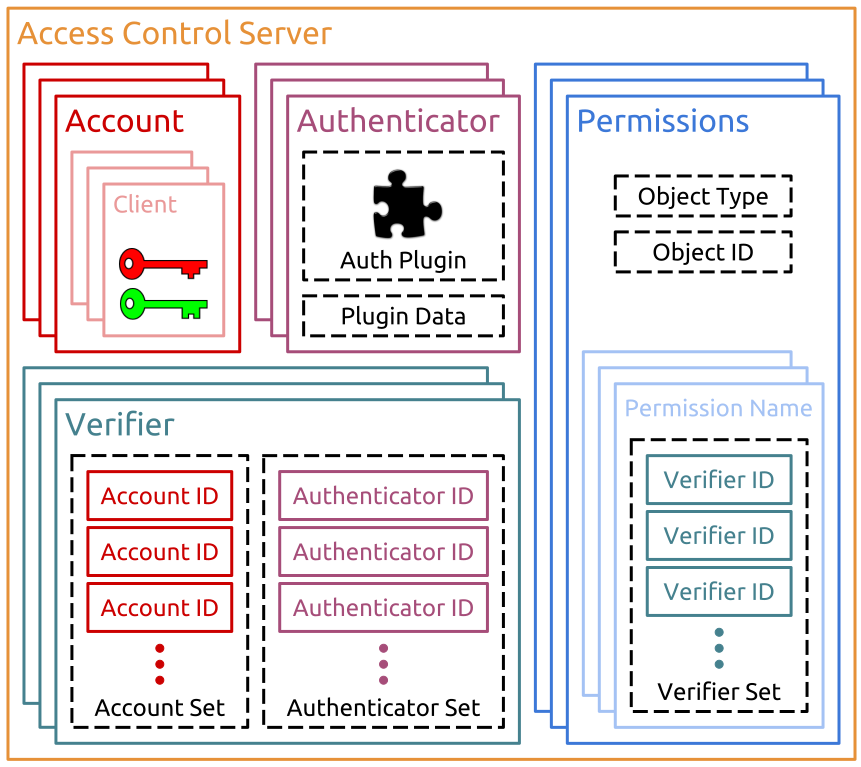
\includegraphics[width=\columnwidth]{./figs/pdf/tutamen-datastructures-ac.pdf}
  \caption{Access Control Server Data Structures}
  \label{fig:tutamen:acstructs}
\end{figure}

In order to track and control access from specific users - the access
control server uses per-user accounts. These accounts are generally
designed to map to individual end-users, but they can be used to track
any singular entity to which one wishes to assign specific access
control privileges. Accounts thus form the basis of controlling and
sharing access to secrets via Tutamen. Within each account are one or
more clients. While accounts map to logically singular access control
entities, clients map to specific devices that will need to make
Tutamen requests. Each account has one or more clients. For example,
Jane Coworker would have a single account with three clients: one for
her laptop, one for her desktop, and one for her phone.

Each client is associated with a single TLS key-pair used to
authenticate the client to the access control server. The access
control server serves as the Certificate Authority administering these
certificates. When a new client is created it generates a local RSA
key and uses this key to generate an X509 Certificate Signing
Request~\cite{rfc5280}. This request is then sent to the access
control server where it awaits approval from an existing client in the
account. If approved, the CSR is used to generate a signed certificate
that is sent back to the new client for use in future access control
server communication. To facilitate bootstrapping new accounts, client
CSRs are also generated and sent with each new account request. These
are atomically approved and associated with the new account --
i.e. the initial client is created in tandem with a new account -- all
subsequent clients are then approved by previously approved clients.

While accounts and clients are used to identify specific
users/entities -- the Tutamen access control server also has
authenticators. Authenticators are modular mechanism used to implement
access control requirements beyond granting access on the basis of
accounts. For example, authenticators can support plugins to perform
additional contextual authentication requirements such as only
allowing access during specific times of day or from requests
originating from specific IP addresses. Authenticators can also be
used to implement out-of-band authentication mechanisms such as
confirming approval for a specific request from a user via text
message or otherwise interfacing with external services to gain
approval.

Accounts and authenticators are combined via verifiers. A verifier
consist of a set of accounts and a set of authenticators. In order to
satisfy a verifier a request must originate from a client in ONE of
the listed accounts and must satisfy ALL of the listed authenticators
plugins. A verifier may contain no Authenticators, in which case
authorization is granted solely on the basis of accounts.

The final component of the Tutamen access control specification are
permission groups. Each permission group corresponds to a specific
object (identified via the combination of an object type and an object
ID) within the Tutamen ecosystem. A permission groups contains one or
more permissions - each corresponding to a specific class of actions
that can be preformed on the corresponding object. Each permission
contains a set of verifiers. In order to be granted a given permission
a request must satisfy at least one of the verifiers in this set.

\subsubsection{Storage Servers}

Tutamen storage servers are responsible for storing all or part of
each Tutamen secret. Figure~\ref{fig:tutamen:storagestructs} shows the
core storage server data structures.

\begin{figure}[th]
  \centering
  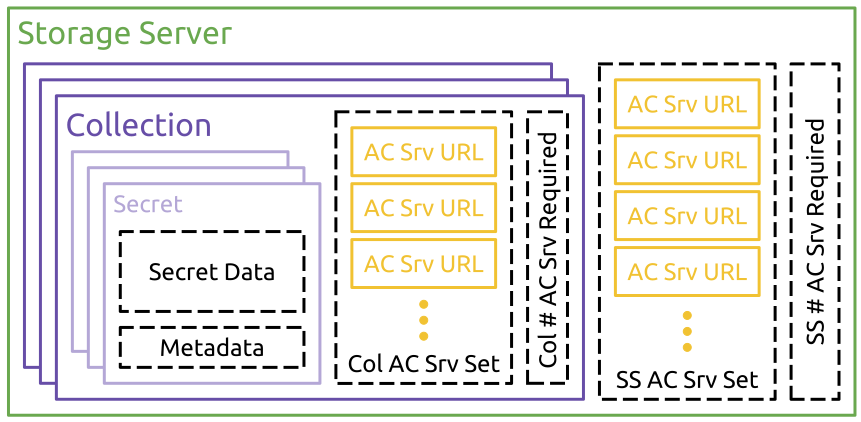
\includegraphics[width=\columnwidth]{./figs/pdf/tutamen-datastructures-storage.pdf}
  \caption{Storage Server Data Structures}
  \label{fig:tutamen:storagestructs}
\end{figure}

The top-level data structure employed by storage servers is a
collection. A collection represents a logical grouping of one or more
secrets (or parts of secrets). Associated with each collection is a
list of one or more access control servers delegated with enforcing
the access control requirements for the collection. Access control
granularity is thus set at the per-collection, not per-secret level. A
collection is also capable of storing a user-provided metadata to aid
in the mapping of collections to the objects for which they store
secrets.

Each collection stores one or more secrets or secret shards. These
secrets consist of the actual secret data the applications leveraging
Tutamen wishes to store as well as any associated user-provided
metadata. Since access control is set at the per-collection level,
secrets inherit their access control characteristics from the
corresponding collection.

% Move to discussion section ?
How best to map secret data to collections is left up to each
applications. This decision is primarily driven by the fact that
access control is preformed on the per-collection level. Thus, if an
applications requires that a set of secrets always have a common set
of access control requirements (e.g. per-sector encryption keys for a
encrypted block device), it make since to group these secrets into a
single collection. Doing so minimizes the complexity of trying to keep
access control requirements synced across multiple secrets and
increases performance by minimizing the number of requests that the
applications must make of the access control server in order to access
multiple secrets in collection. In other cases where each secret
requires its own access control requirements (e.g. per-file encrypting
keys for a sensitive document), it would be appropriate for the
corresponding application to store only a single secret per
collection.

\subsubsection{Access Control Protocol}

Access control servers control access related to both internal
(i.e. access control server) and external (i.e. storage server)
objects by providing signed authorization tokens in response to valid
requests. Each authorization token grants the bearer with specific
permissions related to a specific object. In this manner, access
control servers provide a form of federated access management than
bears some similarities to previously deployed systems such as
Shibboleth~\cite{leandro2012}. Figure~\ref{fig:tutamen:systembase}
shows the basic communication involved in the Tutamen access control
process.

\begin{figure}[th]
  \centering
  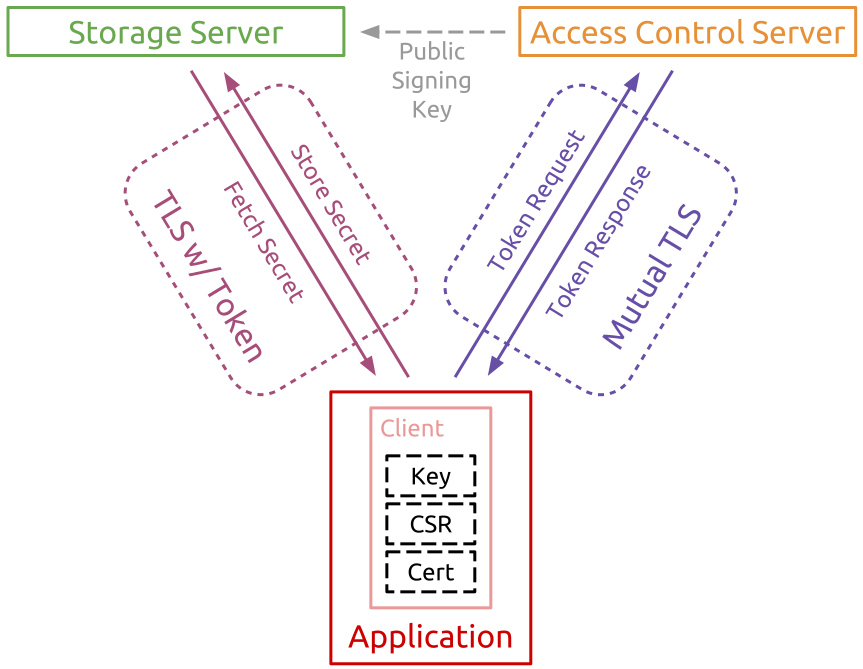
\includegraphics[width=\columnwidth]{./figs/pdf/system-base.pdf}
  \caption{Tutamen System Components}
  \label{fig:tutamen:systembase}
\end{figure}

The access control server generates authorization tokens in response
to a client sending an authorization request. Each authorization
request (and each corresponding token) includes two claims binding it
to a specific object: the object type and the object ID. Each request
also contains a claim that binds it to a specific permission
(e.g. read, write, delete, modify) for the corresponding
object. Authorization requests are further bound to the specific
client making the request (authenticated via mutual-TLS) and to an
expiration time -- after which the token is no longer
valid. Listing~\ref{lst:tutamen:token} shows the structure of Tutamen
access control tokens.

\begin{lstlisting}[float,
    language=JavaScript,
    caption={Authorization Token Contents},
    label=lst:tutamen:token]
{
  "claims":
  {
    "objtype": <object type>,
    "objuid": <object ID>,
    "permission": <object permission>,
    "requesting-client": <client ID>,
    "requesting-account": <account ID>,
    "expiration": <expiration date and time>
  }
  "signature": <AC server signature>
}
\end{lstlisting}

Upon receiving a authorization request from a client, the access
control server looks up the permission group for the corresponding
object (identified via the combination of object type and object ID)
and then loads the verifier set corresponding to the requested
permission. The server then traverses each verifier in this set -
verifying both client membership in one of the accounts listed in the
verifier as well as executing any authenticator plugins required by
the verifier until it finds (or fails to find) a verifier that is
satisfied by the request. If the server is able to verify compliance
with at least one verifier in the permission set it grants the
authorization request and returns a signed authorization token that
includes the object type, object ID, granted permission, expiration
time. The bearer of this token can then present it to either the
access control server or a storage server in order to be granted the
right to perform the class of operations included in the corresponding
permission on the corresponding object.

In this manner, access control servers are responsible both for
granting and verifying authorization requests and signing the
corresponding tokens as well as for verifying tokens accompanying
requests to preform actions on access control server data structures
(e.g. to create or modify verifiers or accounts). Storage servers are
responsible only for verifying tokens accompanying requests to perform
actions on storage server data structures (e.g. to create a collection
or read a secret).

\subsubsection{Distributed Usage}

\begin{figure}[th]
  \centering
  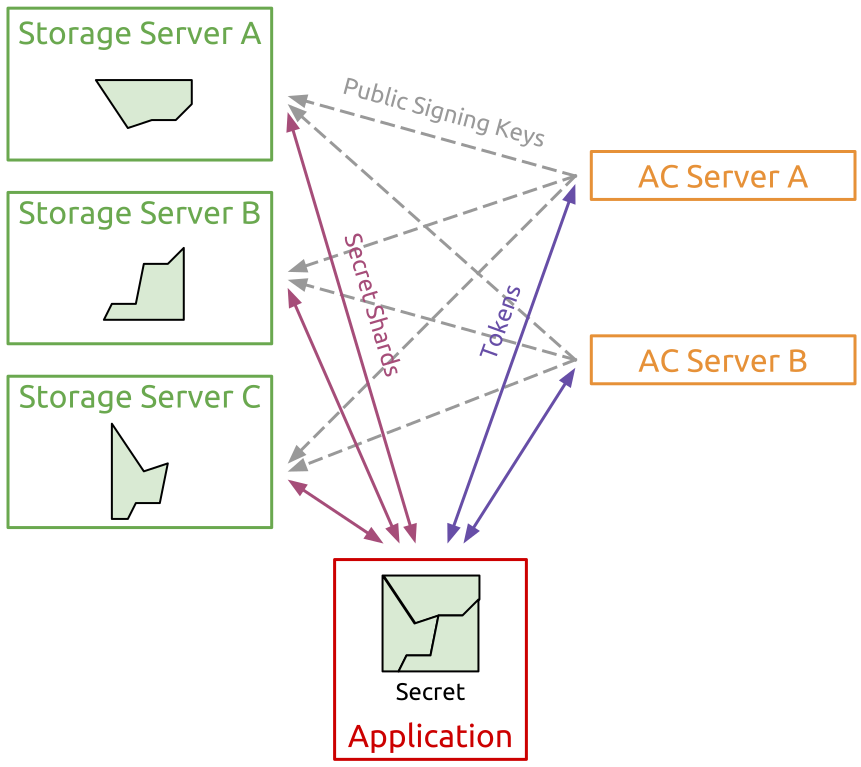
\includegraphics[width=\columnwidth]{./figs/pdf/system-distributed.pdf}
  \caption{Distributed Operation}
  \label{fig:tutamen:systemdistributed}
\end{figure}

% Storage Server Cert Verification Option

\subsubsection{Applications}

% Mapping

\subsubsection{Example}

\subsection{Security and Trust}

\subsubsection{Model}

\subsubsection{Discussion}

\subsection{Implementation}

%%  LocalWords:  Tutamen ACS HTTPS CSR CSRs Authenticators verifiers
%%  LocalWords:  authenticators authenticator objtype objuid
